\documentclass{article}%
\usepackage[T1]{fontenc}%
\usepackage[utf8]{inputenc}%
\usepackage{lmodern}%
\usepackage{textcomp}%
\usepackage{lastpage}%
\usepackage{authblk}%
\usepackage{graphicx}%
%
\title{Differential activation of the inflammasome in THP{-}1 cells exposed to chrysotile asbestos and Libby six{-}mix amphiboles and subsequent activation of BEAS{-}2B cells}%
\author{Kenneth Smith}%
\affil{Department of Neurosurgery, Taichung Veterans General Hospital, Taichung 40705, Taiwan}%
\date{01{-}01{-}2006}%
%
\begin{document}%
\normalsize%
\maketitle%
\section{Abstract}%
\label{sec:Abstract}%
Editor's note: Please read the article in its entirety for more information.\newline%
New research published in the January 1st issue of Cell confirms that a structural change in a protein related to focal adhesion kinase (FAK), found in a patient with non{-}small cell lung cancer, contributes to increased production of a protein called glutamine{-}3{-}androbenzene (GDO) in the tumors. FAK increases the tumorous toxicity in tumors, as well as in blood vessels in the body, and often results in neutropenia and bone marrow toxicity. The study provides the first evidence that progenitor tumors with these mutations are more prone to nutrient degradation, while the expansion of tumor cells may contribute to continued toxicity. The study also points out that there are therapeutic options for patients with these mutations, but they are not targeted for patients with mutated FAK.\newline%
Floyd Resnick and his colleagues, led by Dana Singer, Professor of Medical Genetics at the University of Vermont, conducted a pilot study with patients with advanced cancer treated at Weill Cornell Medical College, New York, using the Cancer Genome Atlas. They found that FAK was elevated in tumor cells with high{-}glurometer concentrations (gluce) and elevated markers for FK that had altered the chemical structure of FAK. Prof. Singer and his team showed that these marker{-}modified tumors contained a thick, silvery skeleton of FAK that strongly resembled the hidden tumors of tumors with normal gamma{-}positive and gamma{-}negative tracers. Their data shows that the Genome Atlas was better than our cells at understanding how the FAK or tumor suppressor cells of the tumor differ from normal cells. The team combined the Genome Atlas and tumor samples from these patients with that of their computerized tumor models to do additional analysis to understand the role that FAK played in the toxicity of some cancers.\newline%
These findings point to the need for targeted therapies that could target tumors with mutations in the FAK pathway to treat cancer. The chemical structure of these tumors may have an influence on which tumor{-}suppression therapies, if any, would be beneficial to them, said Dr. Steven Weisman, Director of the CTRC{-}AACR Premarket, Discovery Institute, MIT, and Cincinnati College of Medicine and Department of Pathology at the University of Texas MD Anderson Cancer Center, partner in the research.\newline%
\#\#\#

%
\subsection{Image Analysis}%
\label{subsec:ImageAnalysis}%


\begin{figure}[h!]%
\centering%
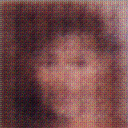
\includegraphics[width=150px]{500_fake_images/samples_5_221.png}%
\caption{A Close Up Of A Person Holding A Cell Phone}%
\end{figure}

%
\end{document}